%template voor een afstudeerwerk in LaTeX
\documentclass[dutch,11pt,cite,titlepage]{report}
%''dutch'' voor splitsing en (in emacs) spellingscontrole
\usepackage{babel}   %voor het geval we ook engels nodig hebben
\usepackage{graphicx} %pakket voor includeren figuren
\usepackage{epsfig}
\usepackage[small]{caption}
\usepackage{url}
\usepackage{subfigure}

\usepackage{scriptie}

\usepackage{pst-bar} % moet (blijkbaar) na het scriptiepakket ingevoegd worden
\usepackage{pst-plot}

\usepackage{mfpic}


% lijst met woorden die LaTeX verkeerd splitst
\hyphenation{vaag-ver-za-me-ling L-vaag-ver-za-me-ling} 

\def\listfigurename{Lijst van figuren}


\begin{document}

\selectlanguage{dutch}


\newcommand{\auteur}{Klaas Bosteels}
\newcommand{\jaar}{2005--2006}
\newcommand{\titel}{Similariteitsgebaseerd rangschikken van afbeeldingen in zoekmachines}
\newcommand{\begeleider}{V. De Witte en S.\ Schulte}
\newcommand{\richting}{licentiaat in de informatica, optie: software-ontwikkeling}

%de volgende lijn kiest de juiste naam van de vakgroepvoorzitter en de promotor
\newcommand{\vakgroep}{Toegepaste Wiskunde en Informatica}
\newcommand{\voorzitter}{prof.\ dr.\ Guido\ Vanden\ Berghe}
\newcommand{\promotor}{prof.\ dr.\ E.\ E.\ Kerre}


%het titelblad vergt hier en daar enkele manuele ingrepen i.v.m.
%spatiering en dergelijke
\begin{titlepage}
\renewcommand{\baselinestretch}{1.1}
\Large
\begin{center}
\mbox{}\\[0cm]%de volgende lijnen genereren het tempeltje
\unitlength 1mm

\epsfysize 4cm \epsfclipon\epsffile{ruglogo.eps}\\
%\begin{picture}(0,20)
%\centering
%\put(0,11){\makebox(0,0)[b]{\font\aula=aula34 {\aula a}}}
%\put(0,6){\makebox(0,0)[b]{\font\futura=futura scaled 1100
%                 {\futura UNIVERSITEIT}}}
%\put(0,2){\makebox(0,0)[b]{\font\futura=futura scaled 1100
%                 {\futura GENT}}}
%\put(0,0){\makebox(0,0)[b]{\rule{21mm}{1pt}}}
%\end{picture}\\
{\Large 
Faculteit \faculteit\\
Vakgroep \vakgroep\\
Voorzitter: \voorzitter
}\\\vfill
\parbox{14 cm}{
{\Huge\bfseries
\begin{center}
\sf\titel
\end{center}
}
}\\\vfill
door\\ 
{\LARGE \auteur}\\[3.3cm]
%we schrijven ``.\"  i.p.v. ``.'' zodat LaTeX weet dat dit een
%afkorting is (gevolgd door kleine spatie) en niet het einde van een
%zin (gevolgd door lange spatie)
%opmerking: ofwel: prof.\ dr.\ I.\ Lemahieu 
%opmerking: ofwel: prof.\ dr.\ ir.\ W.\ Philips
Promotor: \promotor \\
%Co-promotor: \copromotor \\
Scriptiebegeleiders: \begeleider 
\\\vfill
%        In samenwerking met BARCO GRAPHICS\\
Afstudeerwerk ingediend tot het behalen van de graad van\\
%dit moet uiteraard worden aangepast!
\richting\\[1cm]
Academiejaar \jaar
\end{center}
\renewcommand{\baselinestretch}{1}
\end{titlepage}





%%% Local Variables: 
%%% mode: latex
%%% TeX-master: "total"
%%% End: 
 % de titelpagina
\pagenumbering{roman}
\setcounter{page}{1}
\newpage
\thispagestyle{plain}

\section*{Dankwoord}
Graag zou ik iedereen willen bedanken die heeft bijgedragen tot de
verwezenlijking van dit eindwerk. In het bijzonder dank ik:
\begin{itemize}
  \item mijn promotor \promotor\ en mijn begeleiders \begeleider\ voor het scheppen van de
mogelijkheid dit onderzoek te verrichten
  \item \ldots
\end{itemize}
\vfill

%\newpage
%\thispagestyle{plain}
%\vfill

\section*{Toelating tot bruikleen}
De auteur geeft de toelating dit afstudeerwerk voor consultatie 
beschikbaar te stellen en delen van het afstudeerwerk te kopi\"eren voor
persoonlijk gebruik. Elk ander gebruik valt onder de beperkingen van het 
auteursrecht, in het bijzonder met betrekking tot de verplichting de bron 
uitdrukkelijk te vermelden bij het aanhalen van resultaten uit dit 
afstudeerwerk.
\\[1cm]
\auteur\hfill \today
\\[1cm]             %het voorwoord.
\newpage
\thispagestyle{plain}

\begin{center}
{\sf\huge \titel }\\[3mm]
door\\
{\Large\auteur{}} \\
\end{center}
\noindent Afstudeerwerk ingediend tot het behalen van de graad van
\richting
\vspace{3mm}\\
Academiejaar \jaar
\vspace{3mm}\\
\noindent Universiteit Gent\\
Faculteit Wetenschappen\\
\vspace{3mm}\\
\noindent Promotor: \promotor\\
\noindent Scriptiebegeleiders: \begeleider\\
%\noindent Co-promotor: \copromotor\\
\vfill

%\noindent {\bf\Large Samenvatting}\\[1mm]
\section*{Samenvatting}
De exponenti\"ele groei van het internet geeft aanleiding tot een paradoxale
situatie: hoe meer informatie er beschikbaar komt, hoe moeilijker het wordt
om binnen een redelijke tijd accurate informatie te vinden. Zoekmachines zijn momenteel
de meest gebruikte online service, met miljoenen zoekopdrachten per dag. Naast het zoeken
in teksten, groeit de aandacht voor zogenaamde multimedia zoeksystemen. 

In het bijzonder maken de internetgebruikers steeds meer gebruik van zoekmachines die toelaten om 
gigantische collecties van afbeeldingen te doorzoeken. Deze zoekmachines zijn echter nagenoeg 
allemaal tekst-gebaseerd. Dit houdt in dat het zoeken enkel steunt op het vergelijken van opgegeven 
trefwoorden met tekstuele annotaties die toegekend worden aan elke afbeelding. Het hoeft geen
betoog dat het voor de gebruiker niet altijd gemakkelijk is om op deze manier een aanvaarbaar 
resultaat te vinden. Bovendien worden deze annotaties grotendeels automatisch gegenereerd, 
waardoor ze vaak weinig relevant zijn.

De hierboven genoemde problemen kunnen opgelost worden door het zoeken te baseren op de inhoud 
van de afbeeldingen. De bestaande inhoud-gebaseerde systemen kunnen echter nog altijd niet 
toegepast worden op afbeeldingencollecties van dergelijke grote omvang. In deze scriptie geven 
we daarom een alternatief voor deze meer geavanceerde zoeksystemen, waarbij de grootte van 
te doorzoeken collectie geen probleem vormt. 

Dit alternatief kan gezien worden als een uitbreiding van de tekst-gebaseerde zoeksystemen.
De zoekactie begint nog steeds met het specifi\"eren van \'e\'en of meerdere trefwoorden, waarop
het systeem antwoord met een lijst van relevante afbeeldingen. We zorgen er nu echter voor
dat de gebruiker een aantal voorbeeld-afbeeldingen kan kiezen uit deze lijst, waarna het
systeem de zoekresultaten rangschikt op een manier die de gelijkenis met de voorbeelden uitbuit.

Voor het modelleren van de graduele gelijkenis tussen afbeeldingen, maken we gebruik van 
vaagsimilariteitsmaten. Daarnaast zullen we ook nog beroep doen op aggregatieoperatoren,
zowel voor het combineren van verschillende similariteitsmaten als voor het ondersteunen van
meerdere voorbeeld-afbeeldingen. 
%\vspace{5mm}

%\noindent {\bf\Large Trefwoorden}\\[1mm]
\section*{Trefwoorden}
content-based image retrieval, vaagverzamelingen, similariteitsmaten, aggregatieoperatoren

              %samenvatting  van de thesis
\renewcommand{\baselinestretch}{1}

\tableofcontents %genereert de inhoudstafel
%\listoffigures
%\listoftables
%\clearpage

\renewcommand{\baselinestretch}{1}
\pagenumbering{arabic}
\setcounter{page}{1}




\chapter{Inleiding}

Op dit eigenste moment zijn er waarschijnlijk enkele honderden \emph{spiders} actief op internet.
Deze computerprogramma's, die soms ook \emph{robots} of \emph{wanderers} worden genoemd, reizen
het internet rond om bepaalde documenten -- in het bijzonder afbeeldingen -- te localiseren. Deze 
documenten worden ge\"indexeerd in een databank, die dan doorzocht kan worden door een zoekmachine. 

Zoekmachines zoals \emph{Google}\footnote{\url{http://www.google.com}} en 
\emph{Yahoo}\footnote{\url{http://www.yahoo.com}} hebben op die manier reeds databanken
opgebouwd die meer dan een miljard afbeeldingen bevatten. Het wordt bijgevolg steeds belangrijker
om manieren te zoeken om deze gigantische collecties van afbeeldingen op een effeci\"ente wijze
te doorzoeken.


\section{Text-based image retrieval}

Nagenoeg alle bestaande zoekmachines bieden \emph{text-based image retrieval} (TBIR) aan. Hierbij
wordt elke afbeelding voorzien van tekstuele annotaties, zoals bijvoorbeeld de 
bestandsnaam of woorden uit de webpagina waarin de afbeelding gebruikt wordt. Deze annotaties
kunnen dan gebruikt worden voor het indexeren van de afbeeldingen in de databank.


\section{Content-based image retrieval}

Omdat de tekst-gebaseerde aanpak in de praktijk dikwijls tekort schiet, is men op zoek gegaan 
naar manier om het zoeken te baseren op de visuele inhoud van de afbeeldingen. Bij 
\emph{content-based image retrieval} (CBIR) maakt men gebruik van een proces dat 
\emph{(visual) feature extraction} genoemd wordt. Dit proces zet een afbeelding om in een 
\emph{feature vector}. Met behulp van multidimensionale indexering kan men deze kenmerkenvector
dan gebruiken als alternatief voor de tekstuele annotaties bij TBIR.


\section{Similariteitsgebaseerd rangschikken}

Door hun grote complexiteit is het vrijwel onmogelijk om \emph{content-based image retrial systems} 
(CBIRSs) te gebruiken voor het doorzoeken van zeer omvangrijke databanken. 

\chapter{Wiskundige fundamenten}

In dit hoofdstuk introduceren we eerst enkele basisbegrippen uit de vaagverzamelingenleer. 
Daarna volgt een overzicht van de vaagsimilariteitsmaten en aggregatieoperatoren waarvan
we later gebruik zullen maken. We hebben dit deel van deze scriptie bewust zo 
bondig mogelijk gehouden. Voor meer informatie verwijzen
we naar \cite{kerre:vaagmodellen}, \cite{vanderweken:similariteitsmaten} en 
\cite{victor:aggregatieoperatoren}.


\section{Basisbegrippen uit de vaagverzamelingenleer}

\subsection{Posets en tralies}
\label{sectie:posets_en_tralies}

In tegenstelling tot de meeste andere gebieden van de wiskunde, wordt in de theorie der 
vaagverzamelingen het begrip ``orde'' ten volle ge\"exploreerd \cite{kerre:vaagmodellen}. Daarom beginnen we deze 
sectie met het defini\"eren van twee ordestructuren: \emph{partieel geordende verzameling} 
(\emph{poset}) en \emph{tralie}. We maken bovendien van de gelegenheid gebruik om enkele 
belangrijke begrippen in verband met posets te introduceren. 

\begin{definitie}
Een partieel geordende verzameling (poset) is een koppel $(P,\le)$ bestaande uit een niet-ledige
verzameling $P$ en een binaire relatie $\le$ over $P$ die reflexief, antisymmetrisch en 
transitief is:
\begin{itemize}
  \item[(P.1)] $(\forall x \in P)(x \le x)$
  \item[(P.2)] $(\forall (x,y) \in P^2)(x \le y \land y \le x \Rightarrow x = y)$
  \item[(P.3)] $(\forall (x,y,z) \in P^3)(x \le y \land y \le z \Rightarrow x \le z)$
\end{itemize}
De relatie $\le$ wordt een (parti\"ele) orderelatie over $P$ genoemd.
\end{definitie} 
\begin{definitie}
Zij $(P,\le)$ een poset en $A \subseteq P$. Een element $b$ van $P$ is een maximaal element
van $A$ als en slechts als $b \in A$ en $(\forall x \in A)(b \le x \Rightarrow x = b)$. 
\end{definitie}
\begin{definitie}
Zij $(P,\le)$ een poset en $A \subseteq P$. Een element $b$ van $P$ is een minimaal element
van $A$ als en slechts als $b \in A$ en $(\forall x \in A)(x \le b \Rightarrow x = b)$. 
\end{definitie}
\begin{definitie}
Zij $(P,\le)$ een poset en $A \subseteq P$. Een element $b$ van $P$ is een bovengrens voor $A$
als en slechts als $(\forall a \in A)(a \le b)$. Als bovendien geldt $b \in A$, dan noemen
we $b$ het grootste element van $A$. De kleinste bovengrens voor $A$ is het
supremum voor $A$.
\end{definitie}
\begin{definitie}
Zij $(P,\le)$ een poset en $A \subseteq P$. Een element $b$ van $P$ is een ondergrens voor $A$
als en slechts als $(\forall a \in A)(b \le a)$. Als bovendien geldt $b \in A$, dan noemen
we $b$ het kleinste element van $A$. De grootste ondergrens voor $A$ is het
infimum voor $A$.
\end{definitie}
\begin{definitie}
Een poset $(L,\le)$ waarin elk doubleton een supremum en een infimum bezit, noemt men een tralie 
(lattice). Als elke niet-ledige deelverzameling van $L$
een supremum en een infimum bezit, dan is $(L, \le)$ een complete tralie.
\end{definitie}
% ALTERNATIEVE DEFINITIE VAN TRALIE
%% enkele nieuwe commando's die we verder in deze sectie nodig zullen hebben
%\newcommand{\dotand}{\ensuremath{\mathaccent\ldotp\land}}
%\newcommand{\dotor}{\ensuremath{\mathaccent\cdotp\lor}}
%\begin{definitie}
%Een algebra\"ische structuur $(L,\dotor,\dotand)$ bestaande uit een niet-ledige
%verzameling $L$ en twee binaire bewerkingen op $L$ wordt een tralie genoemd als en slechts als
%voor elke $a$, $b$ en $c$ uit $L$ geldt:
%\begin{itemize}
%  \item[(L.1)] $a \dotand a = a$ en $a \dotor a = a$
%  \item[(L.2)] $a \dotand b = b \dotand a$ en $a \dotor b = b \dotor a$
%  \item[(L.3)] $a \dotand (b \dotand c) = (a \dotand b) \dotand c$ en $a \dotor (b \dotor c) = (a \dotor b) \dotor c$
%  \item[(L.4)] $a \dotand (a \dotor b) = a$ en $a \dotor (a \dotand b) = a$
%\end{itemize}
%\end{definitie}

\subsection{Vaagverzamelingen}

Het \emph{universum} is de collectie van alle mogelijke elementen (bijvoorbeeld de
natuurlijke getallen). Een verzameling bevat bepaalde elementen uit dat universum (bijvoorbeeld de 
verzameling van de priemgetallen). 

In het geval van een \emph{scherpe (deel)verzameling} behoort elk 
element uit het universum wel of niet tot de verzameling. Andere mogelijkheden zijn er
niet. Een dergelijke verzameling kan bijgevolg 
gerepresenteerd worden door een \emph{karakteristieke afbeelding}, die elk element uit het 
universum afbeeldt op 0 of 1. Dat getal wordt de \emph{lidmaatschapsgraad} van het element 
in kwestie genoemd. De klasse van scherpe verzamelingen in een universum $X$ stellen we voor door 
$\mathcal{P}(X)$.
\begin{definitie}
Zij $X$ een universum. De karakteristieke afbeelding $\mu_A$ van een scherpe verzameling $A$ in $X$
wordt gedefinieerd als de $X - \{0,1\}$ afbeelding:
\begin{displaymath}
\begin{array}{lllll}
\mu_A: 	& X & \to 		& \{0,1\}	& \\
		& x & \mapsto 	& 1,		& \textrm{ als } x \in A \\
		& x & \mapsto 	& 0,		& \textrm{ als } x \notin A
\end{array}
\end{displaymath}
\end{definitie}

Bij een \emph{vaagverzameling} kunnen alle waarden tussen 0 en 1 als lidmaatschapsgraad 
voorkomen. De ``karakteristieke'' afbeelding is in dat geval dus een $X - [0,1]$ afbeelding:
\begin{definitie}
Zij $X$ een universum. Een vaagverzameling $A$ in $X$ wordt gekarakteriseerd door een $X - [0,1]$
afbeelding  $\mu_A$:
\begin{displaymath}
\begin{array}{lllll}
\mu_A: 	& X & \to 		& [0,1]	& \\
		& x & \mapsto 	& \mu_A(x),		& \forall x \in A
\end{array}
\end{displaymath}
\end{definitie}
\noindent
Een element $x \in X$ behoort dus tot de vaagverzameling $A$ met lidmaatschapsgraad $\mu_A(x)$.
Voor de eenvoud noteren we in het vervolg $\mu_A(x)$ steeds als $A(x)$. We maken
met andere woorden geen onderscheid tussen de vaagverzameling en de 
lidmaatschapsfunctie. Voor de klasse van vaagverzamelingen in een universum $X$ gebruiken we
de notatie $\mathcal{F}(X)$.

De \emph{drager} en de \emph{kern} van een vaagverzameling zijn twee belangrijke begrippen: 
\begin{definitie}
De drager van een vaagverzameling $A$ in $X$ wordt gedefinieerd als:
\begin{displaymath}
supp\ A = \{x \in X \mid A(x) > 0\} 
\end{displaymath}
\end{definitie}
\begin{definitie}
De kern van een vaagverzameling $A$ in $X$ wordt als volgt gedefinieerd:
\begin{displaymath}
ker\ A = \{x \in X \mid A(x) = 1\}
\end{displaymath}
\end{definitie}
\noindent
Ook het begrip \emph{cardinaliteit} speelt vaak een belangrijke rol. De cardinaliteit van een 
eindige scherpe verzameling wordt gegeven door het aantal elementen in die verzameling. 
Dat concept kan uitgebreid worden naar vaagverzamelingen door gebruik te maken van het begrip 
\emph{sigma count}:
\begin{definitie}
De sigma count van een vaagverzameling $A$ met eindige drager in een universum $X$ wordt
gedefinieerd door:
\begin{displaymath}
|A|=\sum_{x \in X} A(x)
\end{displaymath}
\end{definitie}

\subsection{Bewerkingen op vaagverzamelingen}
\label{sectie:bew_op_vaagverz}

We beginnen met het defini\"eren van de begrippen \emph{negator}, \emph{conjunctor} en 
\emph{disjunctor}. Die operatoren zijn uitbreidingen van de klassieke logische operatoren
$\lnot$ (negatie), $\land$ (conjunctie) en $\lor$ (disjunctie).
\begin{definitie}
Een negator $\mathcal{N}$ op $[0,1]$ is een dalende $[0,1] - [0,1]$ afbeelding die voldoet
aan de randvoorwaarden $\mathcal{N}(0)=1$ en $\mathcal{N}(1)=0$. 
\end{definitie}
\begin{definitie}
Een conjunctor $\mathcal{C}$ op $[0,1]$ is een stijgende $[0,1]^2 - [0,1]$ afbeelding die voldoet aan de
randvoorwaarden $\mathcal{C}(0,0)=\mathcal{C}(0,1)=\mathcal{C}(1,0)=0$ en $\mathcal{C}(1,1)=1$. 
Als een conjunctor voldoet aan 
$(\forall a \in [0,1])(\mathcal{C}(1,a)=\mathcal{C}(a,1)=a)$ dan is het een semi-norm.
Een driehoeksnorm (t-norm) is een commutatieve en associatieve semi-norm.
\end{definitie}
\begin{definitie}
Een disjunctor $\mathcal{D}$ op $[0,1]$ is een stijgende $[0,1]^2 - [0,1]$ afbeelding die voldoet
aan de randvoorwaarden $\mathcal{D}(1,0)=\mathcal{D}(0,1)=\mathcal{D}(1,1)=1$ en 
$\mathcal{D}(0,0)=0$. Als een disjunctor voldoet aan 
$(\forall a \in [0,1])(\mathcal{D}(0,a)=\mathcal{D}(a,0)=a)$ dan is het een semi-conorm.
Een driehoeksconorm (t-conorm) is een commutatieve en associatieve semi-conorm.
\end{definitie}

De meest gebruikte negator is de standaardnegator $N_s$. Het minimum $T_M$ en het algebra\"isch 
product $T_P$ zijn veelgebruikte t-normen. Bij de t-conormen zijn het maximum $S_M$ en de
probabilistische som $S_P$ dan weer populaire mogelijkheden. Die operatoren worden als 
volgt gedefinieerd:
%\begin{displaymath}
%\begin{array}{r@{\quad=\quad}l}
\begin{align*}
N_s(x) &= 1 - x \\
T_M(x,y) &= \min \{x,y\} \\
T_P(x,y) &= x \cdot y \\
S_M(x,y) &= \max \{x,y\} \\
S_P(x,y) &= x + y - x \cdot y
\end{align*}
%\end{array}
%\end{displaymath}
voor alle $(x,y)$ in $[0,1]^2$.

We kunnen de bovenstaande operatoren nu gebruiken om de klassieke verzameltechnische bewerkingen 
$co$ (complement), $\cap$ (doorsnede) en $\cup$ (unie) te
veralgemenen tot bewerkingen op vaagverzamelingen.
\begin{definitie}
Het $\mathcal{N}$-complement $co_\mathcal{N} A$ van een vaagverzameling $A$ in $X$ wordt gedefinieerd
door de volgende vaagverzameling in X:
\begin{displaymath}
(co_\mathcal{N} A)(x) = \mathcal{N}(A(x)),
\end{displaymath}
voor alle $x$ in $X$, met $\mathcal{N}$ een negator.
\end{definitie}
\begin{definitie}
De $\mathcal{C}$-doorsnede $A \cap_\mathcal{C} B$ van twee vaagverzamelingen $A$ en $B$ in $X$
wordt gedefinieerd door de volgende vaagverzameling in $X$:
\begin{displaymath}
(A \cap_\mathcal{C} B)(x) = \mathcal{C}(A(x),B(x)),
\end{displaymath}
voor alle $x$ in $X$, met $\mathcal{C}$ een conjunctor.
\end{definitie}
\begin{definitie}
De $\mathcal{D}$-unie $A \cup_\mathcal{D} B$ van twee vaagverzamelingen $A$ en $B$ in $X$ wordt gedefinieerd door de
volgende vaagverzameling in $X$:
\begin{displaymath}
(A \cup_\mathcal{D} B)(x) = \mathcal{D}(A(x),B(x)),
\end{displaymath}
voor alle $x$ in $X$, met $\mathcal{D}$ een disjunctor.
\end{definitie}

In het vervolg van deze scriptie zullen we steeds 
$(\mathcal{N},\mathcal{C},\mathcal{D})=(N_s,T_M,S_M)$ kiezen. We voeren daarom de volgende
verkorte notaties in:
\begin{align*}
A^c 			&= co_{N_s} A \\
A \cap B 		&= A \cap_{T_M} B \\
A \cup B		&= A \cup_{S_M} B \\
A \setminus B  	&= A \cap B^c \\
A \triangle B 	&= (A \setminus B) \cup (B \setminus A)
\end{align*}
waarbij $A$ en $B$ vaagverzamelingen in een zelfde universum zijn.


\subsection{L-vaagverzamelingen}

Het begrip vaagverzameling kan op zijn beurt nog eens uitgebreid worden tot 
\emph{L-vaagverzameling}. Die uitbreiding is gebaseerd op het concept \emph{tralie}
uit sectie~\ref{sectie:posets_en_tralies}.
\begin{definitie}
Zij $X$ een universum en $(L,\le)$ een complete tralie. Een L-vaagverzameling $A$ in $X$ wordt
gekarakteriseerd door een $X - L$ afbeelding $\mu_A$:
\begin{displaymath}
\begin{array}{lllll}
\mu_A: 	& X & \to 		& L	& \\
		& x & \mapsto 	& \mu_A(x),		& \forall x \in A
\end{array}
\end{displaymath}
\end{definitie}
\noindent
De klasse van L-vaagverzamelingen in een universum $X$ stellen we voor door 
$\mathcal{F}_L(X)$. Merk op dat die klasse zich herleidt tot $\mathcal{F}(X)$ voor $L = [0,1]$.

\subsection{Bewerkingen op L-vaagverzamelingen}

De begrippen \emph{negator}, \emph{conjunctor} en 
\emph{disjunctor} kunnen uitgebreid worden naar L-vaag\-ver\-za\-me\-ling\-en. Dat heeft als 
gevolg dat de veralgemeende verzameltechnische bewerkingen $co$, $\cap$ en 
$\cup$ uit \ref{sectie:bew_op_vaagverz} eveneens toepasbaar zijn op L-vaagverzamelingen.
We geven hieronder de definities van die uitbreidingen.
Hierbij is $(L,\le)$ een complete tralie die $l$ als kleinste en $u$ als grootste element heeft.
\begin{definitie}
Een negator $\mathcal{N}$ op $L$ is een dalende $L - L$ afbeelding die voldoet
aan de randvoorwaarden $\mathcal{N}(l)=u$ en $\mathcal{N}(u)=l$. 
\end{definitie}
\begin{definitie}
Een conjunctor $\mathcal{C}$ op $L$ is een stijgende $L^2 - L$ afbeelding die voldoet aan de
randvoorwaarden $\mathcal{C}(l,l)=\mathcal{C}(l,u)=\mathcal{C}(u,l)=l$ en $\mathcal{C}(u,u)=u$. 
Als een conjunctor voldoet aan 
$(\forall a \in L)(\mathcal{C}(u,a)=\mathcal{C}(a,u)=a)$ dan is het een semi-norm.
Een driehoeksnorm (t-norm) is een commutatieve en associatieve semi-norm.
\end{definitie}
\begin{definitie}
Een disjunctor $\mathcal{D}$ op $L$ is een stijgende $L^2 - L$ afbeelding die voldoet
aan de randvoorwaarden $\mathcal{D}(u,l)=\mathcal{D}(l,u)=\mathcal{D}(u,u)=u$ en 
$\mathcal{D}(l,l)=l$. Als een disjunctor voldoet aan 
$(\forall a \in L)(\mathcal{D}(l,a)=\mathcal{D}(a,l)=a)$ dan is het een semi-conorm.
Een driehoeksconorm (t-conorm) is een commutatieve en associatieve semi-conorm.
\end{definitie}

\section{Vaagsimilariteitsmaten}
\label{sectie:vaagsimilariteitsmaten}

Het nagaan van de graduele gelijkenis tussen twee vaagverzamelingen -- of tussen twee objecten die 
identificeerbaar zijn met vaagverzamelingen -- kan aan de hand van \emph{vaagsimilariteitsmaten}. 
Een dergelijke similariteitsmaat voor het vergelijken van twee vaagverzamelingen in een 
universum $X$, is niets meer dan een vaagverzameling in $\mathcal{F}(X) \times \mathcal{F}(X)$. De 
lidmaatschapsgraad van een koppel $(A,B) \in (\mathcal{F}(X))^2$ nadert daarbij naar 1 naarmate 
de similariteit tussen de vaagverzamelingen $A$ en $B$ toeneemt.

In \cite{vanderweken:similariteitsmaten} worden er 32 vaagsimilariteitsmaten voorgesteld: $M_1$, $M_2$,
$M_3$, $M_4$, $M_5$, $M_{5c}$, $M_6$, $M_{6c}$, $M_7$, $M_{7c}$, $M_8$, $M_{8c}$, $M_9$, $M_{9c}$,
$M_{10}$, $M_{10c}$, $M_{11}$, $M_{11c}$, $M_{12}$, $M_{13}$, $M_{14a}$, $M_{14b}$, $M_{14c}$, 
$M_{16e}$, $M_{16h}$, $M_{17a}$, $M_{17b}$, $M_{I_3}$, $M_{I_{3c}}$, $M_{18c}$, $M_{20}$ en $M_{20c}$.
We gaan die echter niet allemaal gebruiken. Vooreerst beperken we ons voor
$$
M_1(A,B) = 1 - \left(\frac{1}{|X|} \sum_{x \in X} | A(x) - B(x)|^r\right)^\frac{1}{r} \textrm{ met } 
r \in \{1,2,3,\ldots\}
$$ tot de keuzes
$r=1,2,4$. De overeenkomstige similariteitsmaten noemen we $M_{1a}$, $M_{1b}$ en $M_{1c}$. Vermits
$M_{1a}=M_{18c}$ hoeven we $M_{18c}$ dan niet meer te beschouwen. 
Bovendien zullen we ons enkel
toespitsen op de maten die rechtstreeks uitbreidbaar zijn naar L-vaagverzamelingen met $L=[0,1]^3$. 
Dit houdt in dat we enkel de maten beschouwen die op evidente wijze kunnen veralgemeend worden naar
vaagverzamelingen in $\mathcal{F}_L(X) \times \mathcal{F}_L(X)$. De details van die
uitbreiding behandelen we in \ref{sectie:pixelgeb_kleurbeelden}. 

Zo komen we uiteindelijk tot
de similariteitsmaten die worden weergegeven in tabel~\ref{tab:similatiteitsmaten}. 
Alle vaagsimilariteitsmaten uit die tabel zijn reflexief en symmetrisch. Dat wil zeggen dat 
voor elke maat $M$ geldt: $M(A,A)=1$ en $M(A,B)=M(B,A)$. 

\begin{table}[tbp]
\begin{center}
\begin{tabular}{|l|}
\hline
\\[1pt]
$
\begin{array}{r@{\ }c@{\ }l}
\displaystyle M_{1a}(A,B) & = & \displaystyle 1-\frac{1}{|X|}\sum_{x \in X} | A(x) - B(x) | \\
\displaystyle M_{1b}(A,B) & = & \displaystyle 1-\left(\frac{1}{|X|}\sum_{x \in X} | A(x) - B(x) |^2\right)^\frac{1}{2} \\
\displaystyle M_{1c}(A,B) & = & \displaystyle 1-\left(\frac{1}{|X|}\sum_{x \in X} | A(x) - B(x) |^4\right)^\frac{1}{4} \\
\end{array}
\begin{array}{r@{\ }c@{\ }l}
\displaystyle M_2(A,B) & = & \displaystyle 1 - \max_{x \in X} | A(x) - B(x) | \\[10pt]
\displaystyle M_3(A,B) & = & \displaystyle 1 - \frac{\displaystyle \sum_{x \in X} | A(x) - B(x) |}{\displaystyle |A| + |B|} \\
\end{array}
$
\\
\\[1pt]
\hline
\\[1pt]
$
\begin{array}{r@{\ }c@{\ }l}
\displaystyle M_5(A,B) & = & \displaystyle \frac{\min \{|A|,|B|\}}{\max \{|A|,|B|\}} \\[10pt]
\displaystyle M_{5c}(A,B) & = & \displaystyle \frac{\min \{|A^c|,|B^c|\}}{\max \{|A^c|,|B^c|\}} \\[10pt]
\displaystyle M_6(A,B) & = & \displaystyle \frac{|A \cap B|}{|A \cup B|} \\[10pt]
\displaystyle M_{6c}(A,B) & = & \displaystyle \frac{|A^c \cap B^c|}{|A^c \cup B^c|} \\[10pt]
\displaystyle M_7(A,B) & = & \displaystyle \frac{|A \cap B|}{\max \{|A|,|B|\}} \\[10pt]
\displaystyle M_{7c}(A,B) & = & \displaystyle \frac{|A^c \cap B^c|}{\max \{|A^c|,|B^c|\}} \\[10pt]
\displaystyle M_8(A,B) & = & \displaystyle \frac{|A \cap B|}{\min \{|A|,|B|\}} \\[10pt]
\displaystyle M_{8c}(A,B) & = & \displaystyle \frac{|A^c \cap B^c|}{\min \{|A^c|,|B^c|\}} \\[10pt]
\end{array}
\begin{array}{@{\qquad}r@{\ }c@{\ }l}
\displaystyle M_9(A,B) & = & \displaystyle \frac{\min \{|A|,|B|\}}{|A \cup B|} \\[10pt]
\displaystyle M_{9c}(A,B) & = & \displaystyle \frac{\min \{|A^c|,|B^c|\}}{|A^c \cup B^c|} \\[10pt]
\displaystyle M_{10}(A,B) & = & \displaystyle \frac{\max \{|A|,|B|\}}{|A \cup B|} \\[10pt]
\displaystyle M_{10c}(A,B) & = & \displaystyle \frac{\max \{|A^c|,|B^c|\}}{|A^c \cup B^c|} \\[10pt]
\displaystyle M_{11}(A,B) & = & \displaystyle \frac{\min \{|A \setminus B|,|B \setminus A|\}}{\max \{|A \setminus B|,|B \setminus A|\}} \\[10pt]
\displaystyle M_{11c}(A,B) & = & \displaystyle \frac{\min \{|(A \setminus B)^c|,|(B \setminus A)^c|\}}{\max \{|(A \setminus B)^c|,|(B \setminus A)^c|\}} \\[10pt]
\displaystyle M_{12}(A,B) & = & \displaystyle \frac{|(A \triangle B)^c|}{\max \{|(A \setminus B)^c|,|(B \setminus A)^c|\}} \\[10pt]
\displaystyle M_{13}(A,B) & = & \displaystyle \frac{|(A \triangle B)^c|}{\min \{|(A \setminus B)^c|,|(B \setminus A)^c|\}}
\end{array}
$
\\
\\[1pt]
\hline
\\[1pt]
$
\begin{array}{r@{\ }c@{\ }l}
\displaystyle M_{I_3}(A,B) & = & \displaystyle \frac{|(A \cap B) \cap (A^c \cap B^c)|}{|(A \cup B) \cap (A^c \cup B^c)|}
\end{array}
\begin{array}{@{\qquad}r@{\ }c@{\ }l}
\displaystyle M_{I_{3c}}(A,B) & = & \displaystyle \frac{|(A^c \cap B^c) \cup (A \cap B)|}{|(A^c \cup B^c) \cup (A \cup B)|}
\end{array}
$
\\
\\[1pt]
\hline
\end{tabular}
\caption{\label{tab:similatiteitsmaten}De vaagsimilariteitsmaten die we gaan gebruiken.}
\end{center}
\end{table}



\section{Aggregatieoperatoren} 

\chapter{Similariteitsmaten voor beelden}

Een similariteitsmaat voor beelden is een maat die de gelijkenis tussen twee gegeven
beelden uitdrukt als een getal in het eenheidsinterval $[0,1]$. Dat getal nadert naar 1
naarmate de gelijkenis groter is. Bijgevolg kunnen we een dergelijke maat gebruiken om
een lijst van zoekresultaten te herordenen volgens similariteit met een bepaald 
voorbeeld uit die lijst. 

We construeren een similariteitsmaat voor beelden in twee stappen. Eerst identificeren we
een beeld, al dan niet rechtstreeks, met een (L-)vaagverzameling. Daarna maken we gebruik van
de vaagsimilariteitsmaten uit \ref{sectie:vaagsimilariteitsmaten} om die (L-)vaagverzamelingen te
vergelijken. 

In het vervolg van deze scriptie bedoelen we met de term ``similariteitsmaat'' steeds
een similariteitsmaat voor beelden. We gebruiken die term dus niet voor een vaagsimilariteitsmaat
op zich, maar wel voor de combinatie van een dergelijke vaagsimilariteitsmaat met een manier om beelden te 
identificeren met (L-)vaagverzamelingen.

\section{Eigenschappen}

In de volgende hoofdstukken construeren we een aantal similariteitsmaten voor beelden. Daarbij 
eisen we dat al onze similariteitsmaten \defin{reflexief} en \defin{symmetrisch} zijn.

\subsection{Reflexiviteit}

Voor twee identieke beelden verwachten we dat een similariteitsmaat $M$ als resultaat $1$
teruggeeft. Met andere woorden, voor een beeld $A$ moet gelden: $M(A,A)=1$.
Die eigenschap heeft als gevolg dat het voorbeeld zich steeds vooraan in
de geordende lijst van zoekresultaten moet bevinden.

\subsection{Symmetrie}

Het resultaat van een similariteitsmaat $M$ wordt verwacht onafhankelijk te zijn van de 
volgorde waarin de beelden aangeboden worden. Voor beelden $A$ en $B$ moet dus gelden:
$M(A,B)=M(B,A)$.

\subsection{Transitiviteit}

De bovenstaande eigenschappen doen denken aan een klassieke equivalentierelatie. Dergelijke
relaties zijn naast reflexief en symmetrisch ook transitief. In 
\cite{zadeh:similarity_relations_and_fuzzy_orderings} definieert Zadeh
de \defin{similariteitsrelatie} als vage uitbreiding van dat scherpe begrip. Als we zouden
afdwingen dat een similariteitsmaat $M$ een similariteitsrelatie is, dan moet $M$ 
\defin{min-transitief}{$\min$-transitief} zijn: voor drie beelden $A$, $B$ en $C$ moet 
$\min\{M(A,B),M(B,C)\} \le M(A,C)$ gelden. Die
eigenschap komt echter niet overeen met de intu\"itieve betekenis van similariteit
\cite{de_cock:on_unsuitable_relations_for_approx_equal, de_cock:why_fuzzy_relations_do_not_resolve_pointcare_paradox}. 
Beschouw bijvoorbeeld de afzonderlijke beelden $A_i$, $i \in \{1,2,\ldots,n\}$, uit \'e\'en sc\`ene van een video. 
Daarbij zullen opeenvolgende beelden doorgaans zeer similair zijn, met andere woorden: 
$M(A_i,A_{i+1}) \approx 1$ voor $i \in \{1,2,\ldots,n-1\}$. Uit de $\min$-transitiviteit
zou dan volgen dat ook $M(A_1,A_n) \approx 1$, terwijl het eerste en het laatste beeld
van een sc\`ene meestal sterk verschillend zijn.   

\section{Evaluatie van performantie}

\subsection{Globale genormaliseerde gemiddelde rang (GGGR)}

Om uit meerdere similariteitsmaten de meest geschikte te kiezen, 
moeten we een manier vinden om een dergelijke maat objectief te beoordelen. 
Dat doen we door, voor een bepaald voorbeeld, elke maat toe te passen op eenzelfde collectie 
van beelden. Vervolgens beoordelen we de zo bekomen rangschikking met behulp van een performantiemaat.

Figuur~\ref{fig:testcollectie} bevat de collectie van beelden die we gaan 
gebruiken. Die collectie bestaat uit een selectie van beelden uit
de \defin{Columbia object image library} \cite{coil-100}, die gegenereerd werd 
door een aantal roterende objecten op bepaalde vaste momenten te fotograferen. 
Onze testcollectie bestaat uit foto's van elf objecten. Van elk object zijn
er zes momentopnames, wat een totaal van $11 \cdot 6 = 66$ beelden geeft.

\begin{figure}[p]
\vspace{5pt}
\centering

\begin{tabular}{cccccc}

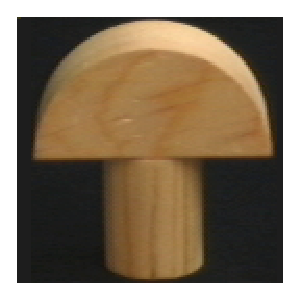
\includegraphics[width=2cm]{coil/beeld-0.eps} &
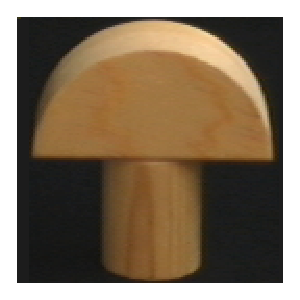
\includegraphics[width=2cm]{coil/beeld-1.eps} &

\includegraphics[width=2cm]{coil/beeld-2.eps} &
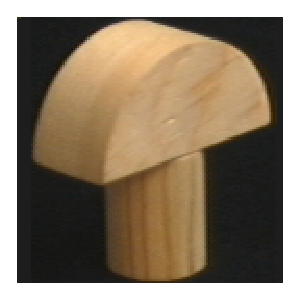
\includegraphics[width=2cm]{coil/beeld-3.eps} &
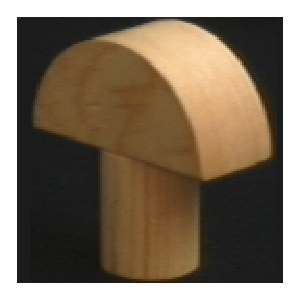
\includegraphics[width=2cm]{coil/beeld-4.eps} &

\includegraphics[width=2cm]{coil/beeld-5.eps} \\

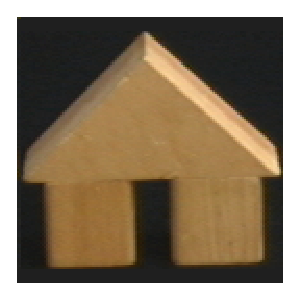
\includegraphics[width=2cm]{coil/beeld-42.eps} &
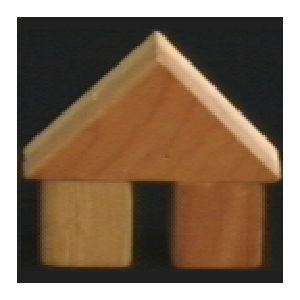
\includegraphics[width=2cm]{coil/beeld-43.eps} &

\includegraphics[width=2cm]{coil/beeld-44.eps} &
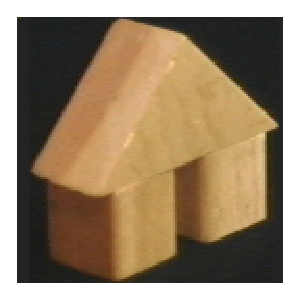
\includegraphics[width=2cm]{coil/beeld-45.eps} &
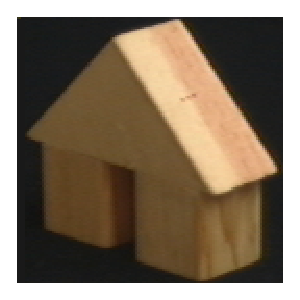
\includegraphics[width=2cm]{coil/beeld-46.eps} &

\includegraphics[width=2cm]{coil/beeld-47.eps} \\


\includegraphics[width=2cm]{coil/beeld-12.eps} &
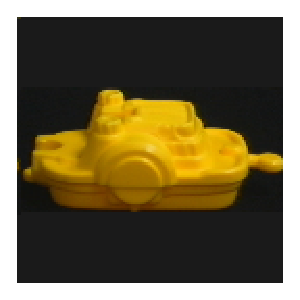
\includegraphics[width=2cm]{coil/beeld-13.eps} &
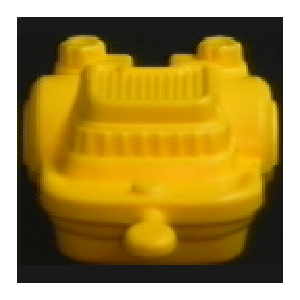
\includegraphics[width=2cm]{coil/beeld-14.eps} &
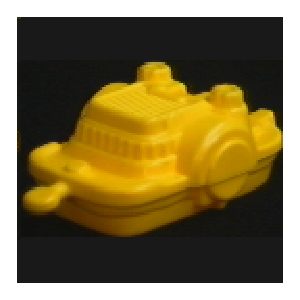
\includegraphics[width=2cm]{coil/beeld-15.eps} &
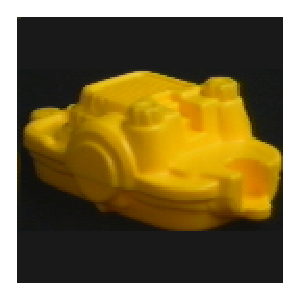
\includegraphics[width=2cm]{coil/beeld-16.eps} &
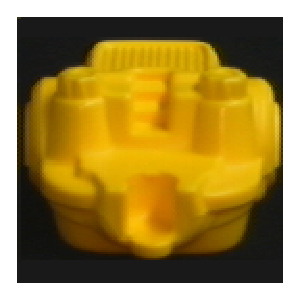
\includegraphics[width=2cm]{coil/beeld-17.eps} \\


\includegraphics[width=2cm]{coil/beeld-18.eps} &

\includegraphics[width=2cm]{coil/beeld-19.eps} &
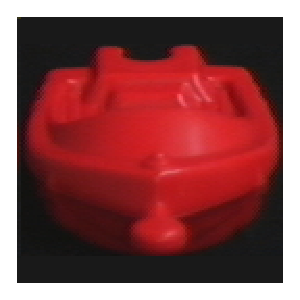
\includegraphics[width=2cm]{coil/beeld-20.eps} &
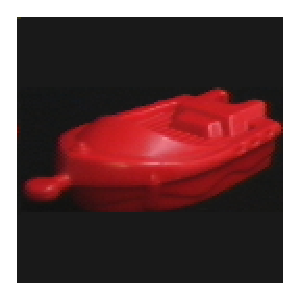
\includegraphics[width=2cm]{coil/beeld-21.eps} &
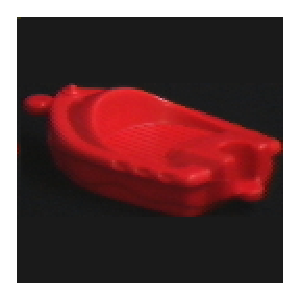
\includegraphics[width=2cm]{coil/beeld-22.eps} &
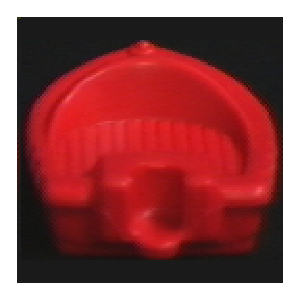
\includegraphics[width=2cm]{coil/beeld-23.eps} \\

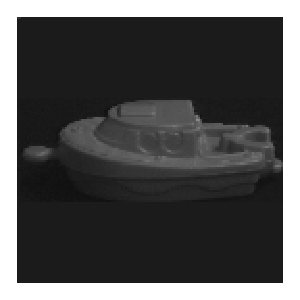
\includegraphics[width=2cm]{coil/beeld-24.eps} &
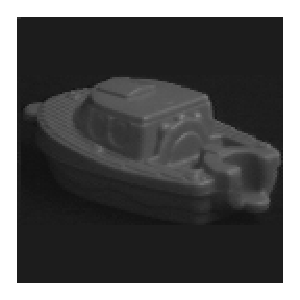
\includegraphics[width=2cm]{coil/beeld-25.eps} &
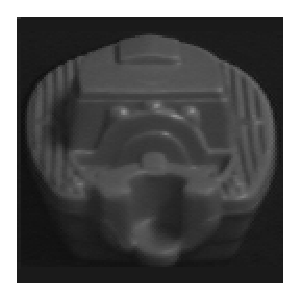
\includegraphics[width=2cm]{coil/beeld-26.eps} &
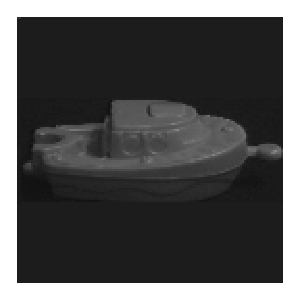
\includegraphics[width=2cm]{coil/beeld-27.eps} &
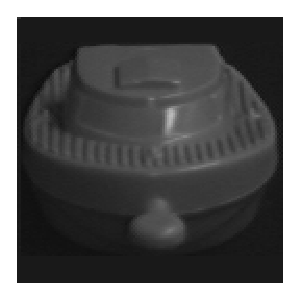
\includegraphics[width=2cm]{coil/beeld-28.eps} &
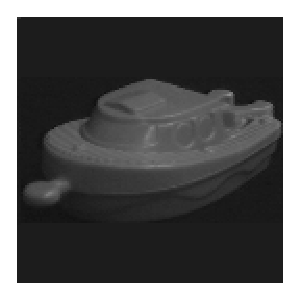
\includegraphics[width=2cm]{coil/beeld-29.eps} \\


\includegraphics[width=2cm]{coil/beeld-54.eps} &

\includegraphics[width=2cm]{coil/beeld-55.eps} &
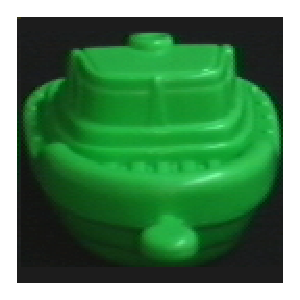
\includegraphics[width=2cm]{coil/beeld-56.eps} &

\includegraphics[width=2cm]{coil/beeld-57.eps} &
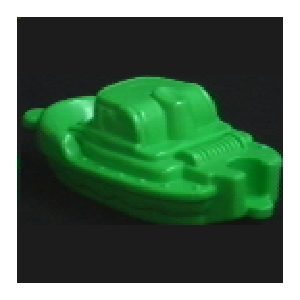
\includegraphics[width=2cm]{coil/beeld-58.eps} &
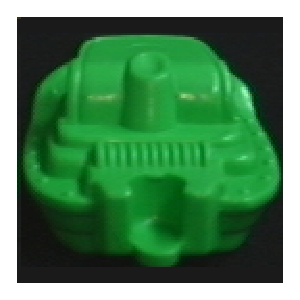
\includegraphics[width=2cm]{coil/beeld-59.eps} \\


\includegraphics[width=2cm]{coil/beeld-30.eps} &
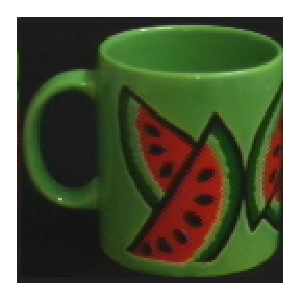
\includegraphics[width=2cm]{coil/beeld-31.eps} &
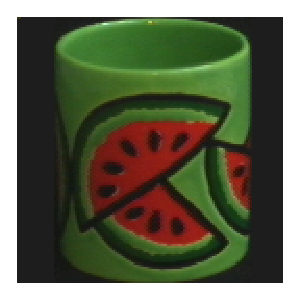
\includegraphics[width=2cm]{coil/beeld-32.eps} &

\includegraphics[width=2cm]{coil/beeld-33.eps} &

\includegraphics[width=2cm]{coil/beeld-34.eps} &

\includegraphics[width=2cm]{coil/beeld-35.eps} \\


\includegraphics[width=2cm]{coil/beeld-36.eps} &

\includegraphics[width=2cm]{coil/beeld-37.eps} &

\includegraphics[width=2cm]{coil/beeld-38.eps} &
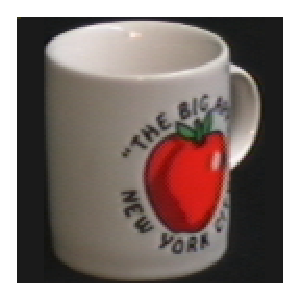
\includegraphics[width=2cm]{coil/beeld-39.eps} &
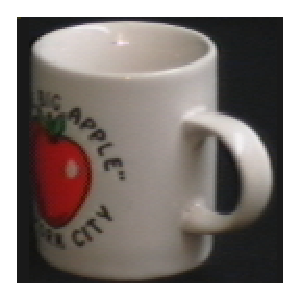
\includegraphics[width=2cm]{coil/beeld-40.eps} &
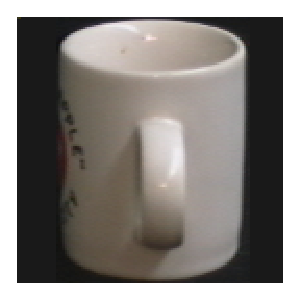
\includegraphics[width=2cm]{coil/beeld-41.eps} \\

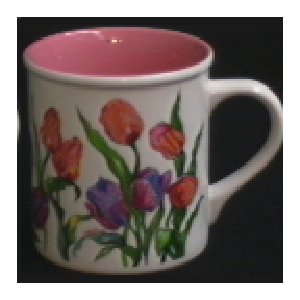
\includegraphics[width=2cm]{coil/beeld-6.eps} &
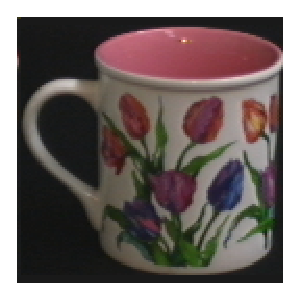
\includegraphics[width=2cm]{coil/beeld-7.eps} &
\includegraphics[width=2cm]{coil/beeld-8.eps} &
\includegraphics[width=2cm]{coil/beeld-9.eps} &
\includegraphics[width=2cm]{coil/beeld-10.eps} &
\includegraphics[width=2cm]{coil/beeld-11.eps} \\

\includegraphics[width=2cm]{coil/beeld-48.eps} &
\includegraphics[width=2cm]{coil/beeld-49.eps} &
\includegraphics[width=2cm]{coil/beeld-50.eps} &
\includegraphics[width=2cm]{coil/beeld-51.eps} &
\includegraphics[width=2cm]{coil/beeld-52.eps} &
\includegraphics[width=2cm]{coil/beeld-53.eps} \\

\includegraphics[width=2cm]{coil/beeld-60.eps} &
\includegraphics[width=2cm]{coil/beeld-61.eps} &
\includegraphics[width=2cm]{coil/beeld-62.eps} &
\includegraphics[width=2cm]{coil/beeld-63.eps} &
\includegraphics[width=2cm]{coil/beeld-64.eps} &
\includegraphics[width=2cm]{coil/beeld-65.eps} \\

\end{tabular}
\vspace{5pt}
\caption{\label{fig:testcollectie}De gebruikte collectie van beelden.}
\end{figure}

Voor het beoordelen van een rangschikking, gebruiken we de \defin{genormaliseerde gemiddelde rang} 
(GGR) \cite{muller:perf_eval}. Die performantiemaat wordt toegepast op een collectie
van $N$ beelden. Voor elk van die beelden bevat de collectie
$N_R$ zogenaamde \defin{relevante beelden}. In het geval van onze testcollectie geldt $N = 66$.
We gaan er in die collectie van uit dat foto's van eenzelfde object relevant zijn ten opzichte
van elkaar: $N_R = 6$. Beschouw nu de vector 
$(r_1,r_2,\ldots,r_{N_R}) \in \{1,2,\ldots,N\}^{N_R}$, waarbij $r_i$ het
rangnummer van het $i$-de relevante beeld voorstelt. De performantiemaat
wordt dan als volgt gedefinieerd:
\begin{definitie}
De genormaliseerde gemiddelde rang wordt gegeven door de volgende afbeelding:
\begin{displaymath}
\begin{array}{lrcl}
\textrm{GGR}: 	& \{1,2,\ldots,N\}^{N_R} & \to 	& [0,1] \\
		& (r_1,r_2,\ldots,r_{N_R}) & \mapsto &
	{\displaystyle\frac{1}{N \cdot N_R}\left[ \left(\sum_{i=1}^{N_R}r_i\right) - \frac{N_R \cdot (N_R + 1)}{2} \right]},\\[15pt]
	& & & \qquad \quad \forall (r_1, r_2, ..., r_{N_R}) \in \{1,2,\ldots,N\}^{N_R}
\end{array}
\end{displaymath}
\end{definitie}
\noindent
Deze maat nadert naar 1 naarmate de performantie slechter wordt.

Tot nu toe hebben we er nog geen rekening mee gehouden dat de performantie van
een similariteitsmaat afhankelijk kan zijn van het gekozen voorbeeld. Dat probleem lossen we
op door de GGR te berekenen voor meerdere voorbeelden en het gemiddelde van de bekomen waarden
te beschouwen. We kiezen daarbij de beelden uit de linker kolom van 
figuur~\ref{fig:testcollectie} als voorbeeld. De waarde die we zo bekomen noemen we de
\defin{genormaliseerde gemiddelde rang!globale}{globale genormaliseerde gemiddelde rang} 
(GGGR). Het is die waarde die we zullen gebruiken
om de performantie van een similariteitsmaat te evalueren. We zullen dus met andere woorden op
zoek gaan naar similariteitsmaten waarvan de GGGR zo klein mogelijk is.

\subsection{Rekentijd}

Voor elke similariteitsmaat die we construeren meten we ook hoe lang het duurt om
de rangschikkingen, die nodig zijn om de GGGR te bepalen, te berekenen. Aan die 
rekentijd hechten we echter niet zoveel belang als aan de GGGR, vermits het in onze
praktische implementatie niet absoluut noodzakelijk is dat de similariteitsmaten zo weinig
mogelijk rekentijd vereisen. De collecties van beelden waarop ze daarbij toegepast worden,
zijn immers beperkt in grootte. Bovendien worden de berekeningen aan de kant van de client
uitgevoerd, waardoor er geen gevaar is voor overbelasting van de server.

Indien we de similariteitsmaten zouden construeren voor een zuiver CBIR-systeem, zoals weergegeven
in figuur~\ref{fig:cbir}, dan zou de rekentijd wel zeer belangrijk zijn. Hoewel het aantal
beelden beperkt wordt door het gebruik van multidimensionale indexering, zal een dergelijk
systeem de similariteitsmaten immers toch nog moeten toepassen op een groot aantal
beelden. Anderzijds laat een zuiver CBIR-systeem wel toe om berekeningen op voorhand te doen
en de resultaten ervan samen met de beelden op te slaan in de databank. Bij het similariteitsgebaseerd
rangschikken van de zoekresultaten is dat niet mogelijk, omdat de databank daarbij niet rechtstreeks
toegankelijk is.

Als we het bepalen van de similariteiten vergelijken met het studeren voor een examen, dan 
heeft de student in het geval van echte CBIR op voorhand meer dan voldoende tijd om de leerstof
te verwerken. Vlak voor het examen is er echter maar net genoeg tijd om alles nog eens 
te herhalen. Bij het similariteitsgebaseerd rangschikken van de zoekresultaten kan er niet vooraf 
gestudeerd worden, maar juist voor het examen heeft de student wel nog enkele dagen ter beschikking 
om alles in te studeren.


\section{Beperken van de rekentijd}
\label{sectie:beperken_rekentijd}

Hoewel de rekentijd voor onze praktische toepassing niet van cruciaal belang is, kan het beperken 
ervan uiteraard geen kwaad. Door toch voldoende aandacht te schenken aan de rekentijd kunnen
we er zelfs voor zorgen dat similariteitsmaten waarvoor we zonder extra inspanning veel te lang zouden 
moeten rekenen, toch nog bruikbaar zijn.

Stel dat $A$ en $B$ twee vaagverzamelingen zijn in een zelfde universum $X$. Het kan dan voorkomen dat 
$X'= supp\ A \cup supp\ B$ veel minder elementen bevat dan $X$. In dat geval kunnen we de rekentijd sterk
reduceren door het bereik van de sommaties in de vaagsimilariteitsmaten te beperken tot $X'$. Doordat
$A(x)=B(x)=0$ voor alle $x \in X \setminus X'$ geldt er dan immers zowel
\begin{align*}
\displaystyle \sum_{x \in X} | A(x) - B(x) | 
&= \displaystyle \sum_{x \in X \setminus X'} | A(x) - B(x) | + \displaystyle \sum_{x \in X'} | A(x) - B(x) | \\
&= \displaystyle \sum_{x \in X \setminus X'} | 0 - 0 | + \displaystyle \sum_{x \in X'} | A(x) - B(x) | \\
&= \displaystyle \sum_{x \in X'} | A(x) - B(x) |
\end{align*}
als $|A| = \sum_{x \in X} A(x) = \sum_{x \in X \setminus X'} 0 + \sum_{x \in X'} A(x) 
= \sum_{x \in X'} A(x)$.
% \begin{displaymath}
% |A| = \sum_{x \in X} A(x) = \sum_{x \in X \setminus X'} A(x) + \sum_{x \in X'} A(x) 
% = \sum_{x \in X \setminus X'} 0 + \sum_{x \in X'} A(x) = \sum_{x \in X'} A(x)
% \end{displaymath}
Wanneer we 
\begin{displaymath}
||A|| = \sum_{x \in X'} A(x)
\end{displaymath} 
defini\"eren, dan geldt dus $|A| = ||A||$ en ook:
\begin{align*}
| A \cap B | 
&= \displaystyle \sum_{x \in X} T_M(A(x),B(x)) & & \\
&= \displaystyle \sum_{x \in X'} T_M(A(x),B(x)) & & (T_M(0,0)=0) \\
&= ||A \cap B|| & & \displaybreak[0] \\ %[5pt]
| A \cup B | 
&= \displaystyle \sum_{x \in X} S_M(A(x),B(x)) & & \\
&= \displaystyle \sum_{x \in X'} S_M(A(x),B(x)) & & (S_M(0,0)=0) \\
&=  ||A \cup B|| & & \displaybreak[0] \\ %[5pt]
| A \setminus B | = | A \cap B^c | 
&= \displaystyle \sum_{x \in X} T_M(A(x),1-B(x)) & & \\
&= \displaystyle \sum_{x \in X'} T_M(A(x),1-B(x)) & & (T_M(0,1-0)=T_M(0,1)=0) \\
&= || A \cap B^c || = ||A \setminus B|| & & %\\[5pt]
\end{align*}
Doordat $T_M(0,1)=0$ en $S_M(0,0)=0$ geldt eveneens
% \begin{align*}
% | A \triangle B | 
% &= | (A \setminus B) \cup (B \setminus A) | & & \\
% &= || (A \setminus B) \cup (B \setminus A) || & & (T_M(0,1)=0 \textrm{ en } S_M(0,0)=0) \\
% &= || A \triangle B || & & \\
% \end{align*}
\begin{displaymath}
| A \triangle B | = | (A \setminus B) \cup (B \setminus A) | = || (A \setminus B) \cup (B \setminus A) || = || A \triangle B ||
\end{displaymath}
% \end{align*}
en uit $T_M(0,1)=0$ volgt dat 
% \begin{align*}
% |(A \cap B) \cap (A^c \cap B^c)| &= ||(A \cap B) \cap (A^c \cap B^c)|| & & (T_M(0,1)=0)\\ %[5pt]
% |(A \cup B) \cap (A^c \cup B^c)| &= ||(A \cup B) \cap (A^c \cup B^c)|| & & (T_M(0,1)=0)
% \end{align*}
$|(A \cap B) \cap (A^c \cap B^c)| = ||(A \cap B) \cap (A^c \cap B^c)||$ en
$|(A \cup B) \cap (A^c \cup B^c)| = ||(A \cup B) \cap (A^c \cup B^c)||$.
Met behulp van de eigenschap
\begin{displaymath}
|A^c| = \sum_{x \in X} (1 - A(x)) = \sum_{x \in X} 1 - \sum_{x \in X} A(x) = |X| - |A|
\end{displaymath}
vinden we bovendien:
\begin{displaymath}
\begin{array}{l@{\ =\ }l@{\ =\ }l@{\ =\ }l}
|A^c \cap B^c| & |(A \cup B)^c| & |X| - |A \cup B| & |X| - ||A \cup B|| \\[4pt]
|A^c \cup B^c| & |(A \cap B)^c| & |X| - |A \cap B| & |X| - ||A \cap B||
\end{array}
\end{displaymath}
\begin{displaymath}
\begin{array}{l@{\ =\ }l@{\ =\ }l}
| (A \setminus B)^c | & |X| - |A \setminus B| & |X| - ||A \setminus B|| \\[4pt]
| (A \triangle B)^c | & |X| - |A \triangle B| & |X| - ||A \triangle B||
\end{array}
\end{displaymath}
\begin{displaymath}
\begin{array}{l@{\ =\ }l@{\ =\ }l}
|(A^c \cap B^c) \cup (A \cap B)| & |((A \cup B) \cap (A^c \cup B^c))^c| & |X| - ||(A \cup B) \cap (A^c \cup B^c)|| \\[4pt]
|(A^c \cup B^c) \cup (A \cup B)| & |((A \cap B) \cap (A^c \cap B^c))^c| & |X| - ||(A \cap B) \cap (A^c \cap B^c)||
\end{array}
\end{displaymath}
We kunnen tabel~\ref{tab:similatiteitsmaten} bijgevolg herschrijven tot tabel~\ref{tab:beperkte_similatiteitsmaten}.
\begin{table}[!bp]
\vspace{10pt}
\centering
\begin{tabular}{l}
%\hline
%\\[1pt]
$
\begin{array}{r@{\ }c@{\ }l}
\displaystyle M_{1a}(A,B) & = & \displaystyle 1-\frac{1}{|X|}\sum_{x \in X'} | A(x) - B(x) | \\
\displaystyle M_{1b}(A,B) & = & \displaystyle 1-\left(\frac{1}{|X|}\sum_{x \in X'} | A(x) - B(x) |^2\right)^\frac{1}{2} \\
\displaystyle M_{1c}(A,B) & = & \displaystyle 1-\left(\frac{1}{|X|}\sum_{x \in X'} | A(x) - B(x) |^4\right)^\frac{1}{4} \\
\end{array}
\begin{array}{r@{\ }c@{\ }l}
\displaystyle M_2(A,B) & = & \displaystyle 1 - \max_{x \in X'} | A(x) - B(x) | \\[10pt]
\displaystyle M_3(A,B) & = & \displaystyle 1 - \frac{\displaystyle \sum_{x \in X'} | A(x) - B(x) |}{\displaystyle ||A|| + ||B||} \\
\end{array}
$
\\
\\[1pt]
\hline
\\[1pt]
$
\begin{array}{r@{\ }c@{\ }l}
\displaystyle M_5(A,B) & = & \displaystyle \frac{\min \{||A||,||B||\}}{\max \{||A||,||B||\}} \\[10pt]
\displaystyle M_{5c}(A,B) & = & \displaystyle \frac{|X|-\max \{||A||,||B||\}}{|X|-\min \{||A||,||B||\}} \\[10pt]
\displaystyle M_6(A,B) & = & \displaystyle \frac{||A \cap B||}{||A \cup B||} \\[10pt]
\displaystyle M_{6c}(A,B) & = & \displaystyle \frac{|X|-||A \cup B||}{|X|-||A \cap B||} \\[10pt]
\displaystyle M_7(A,B) & = & \displaystyle \frac{||A \cap B||}{\max \{||A||,||B||\}} \\[10pt]
\displaystyle M_{7c}(A,B) & = & \displaystyle \frac{|X|-||A \cup B||}{|X|-\min \{||A||,||B||\}} \\[10pt]
\displaystyle M_8(A,B) & = & \displaystyle \frac{||A \cap B||}{\min \{||A||,||B||\}} \\[10pt]
\displaystyle M_{8c}(A,B) & = & \displaystyle \frac{|X|-||A \cup B||}{|X|-\max \{||A||,||B||\}} \\[10pt]
\end{array}
\begin{array}{@{\qquad}r@{\ }c@{\ }l}
\displaystyle M_9(A,B) & = & \displaystyle \frac{\min \{||A||,||B||\}}{||A \cup B||} \\[10pt]
\displaystyle M_{9c}(A,B) & = & \displaystyle \frac{|X| - \max \{||A||,||B||\}}{|X| - ||A \cap B||} \\[10pt]
\displaystyle M_{10}(A,B) & = & \displaystyle \frac{\max \{||A||,||B||\}}{||A \cup B||} \\[10pt]
\displaystyle M_{10c}(A,B) & = & \displaystyle \frac{|X| - \min \{||A||,||B||\}}{|X| - ||A \cap B||} \\[10pt]
\displaystyle M_{11}(A,B) & = & \displaystyle \frac{\min \{||A \setminus B||,||B \setminus A||\}}{\max \{||A \setminus B||,||B \setminus A||\}} \\[10pt]
\displaystyle M_{11c}(A,B) & = & \displaystyle \frac{|X| - \max \{||A \setminus B||,||B \setminus A||\}}{|X| - \min \{||A \setminus B||,||B \setminus A||\}} \\[10pt]
\displaystyle M_{12}(A,B) & = & \displaystyle \frac{|X| - ||A \triangle B||}{|X|-\min \{||A \setminus B||,||B \setminus A||\}} \\[10pt]
\displaystyle M_{13}(A,B) & = & \displaystyle \frac{|X|-||A \triangle B||}{|X|-\max \{||A \setminus B||,||B \setminus A||\}}
\end{array}
$
\\
\\[1pt]
\hline
\\[1pt]
$
\begin{array}{r@{\ }c@{\ }l}
\displaystyle M_{I_3}(A,B) & = & \displaystyle \frac{||(A \cap B) \cap (A^c \cap B^c)||}{||(A \cup B) \cap (A^c \cup B^c)||}
\end{array}
\begin{array}{@{\qquad}r@{\ }c@{\ }l}
\displaystyle M_{I_{3c}}(A,B) & = & \displaystyle \frac{|X| - ||(A \cup B) \cap (A^c \cup B^c)||}{|X|-||(A \cap B) \cap (A^c \cap B^c)||}
\end{array}
$
%\\
%\\[1pt]
%\hline
\end{tabular}
\vspace{10pt}
\caption{\label{tab:beperkte_similatiteitsmaten}De vaagsimilariteitsmaten geschreven met 
sommaties waarvan het bereik beperkt is.}
\end{table}
% beter geen nieuwe paragraaf volgens Valerie
Beschouw bijvoorbeeld $M_{5}$:
\begin{displaymath}
M_{5} = \frac{\min\{|A|,|B|\}}{\max\{|A|,|B|\}} = \frac{\min\{||A||,||B||\}}{\max\{||A||,||B||\}}
\end{displaymath}
Bij de oude formule zijn er eerst $2 \cdot (|X|-1)$ optellingen nodig
om $|A|$ en $|B|$ te berekenen. Daarna moeten de zo bekomen getallen met elkaar vergeleken worden
om $\min\{|A|,|B|\}$ en $\max\{|A|,|B|\}$ te bepalen en moet er tenslotte ook nog \'e\'en deling
uitgevoerd worden. De herschreven vorm vereist $ 2 \cdot (|X'|-1)$ optellingen, \'e\'en vergelijking
en \'e\'en deling. Vermits $|X'| \ll |X|$ impliceert 
dat $2 \cdot (|X'|-1) + 2 \ll 2 \cdot (|X|-1) + 2$, zal de nieuwe formule inderdaad een stuk sneller kunnen 
berekend worden dan de oude als $X'$ veel minder elementen bevat dan $X$. Bovendien zijn de rekentijden
gelijk als $X'=X$. De nieuwe vorm is dus steeds minstens even snel als de oude.

Bij de vaagsimilariteitsmaten die gebruik maken van het complement, boeken we nog meer winst.
We bekijken $M_{5c}$ als voorbeeld. De oorspronkelijke vorm wordt als volgt herschreven:
\begin{align*}
\displaystyle M_{5c}(A,B) = \displaystyle \frac{\min \{|A^c|,|B^c|\}}{\max \{|A^c|,|B^c|\}} 
& = \displaystyle \frac{\min \{|X|-||A||,|X|-||B||\}}{\max \{|X|-||A||,|X|-||B||\}} \\
& = \displaystyle \frac{|X| + \min \{-||A||,-||B||\}}{|X| + \max \{-||A||,-||B||\}} \\
& = \displaystyle \frac{|X| - \max \{||A||,||B||\}}{|X| - \min \{||A||,||B||\}}
\end{align*}
Voor de oude formule zijn er $2\cdot |X|$ aftrekkingen nodig om $A^c$ en $B^c$ te bepalen,
bovenop de $2 \cdot (|X|-1) + 2$ bewerkingen die nodig zijn voor het berekenen van 
%$\min\{|A|,|B|\} / \max\{|A|,|B|\}$. 
de originele vorm van $M_5$. De nieuwe formule daarentegen vereist slechts twee bewerkingen
meer dan de herschreven vorm van $M_5$. Zelfs voor $|X'| = |X|$ zal 
$2 \cdot |X| + 2 \cdot (|X|-1) + 2 = 4 \cdot |X|$ doorgaans een stuk groter zijn dan
$2 \cdot (|X'|-1) + 4 = 2 \cdot |X'| + 2$. Als $|X'| \ll |X|$ dan wordt het verschil in rekentijd
uiteraard nog significanter.

Merk op dat we in de bovenstaande redeneringen enkel gesteund hebben op $T_M(0,0)=T_M(0,1)=0$ en 
$S_M(0,0)=0$. 
De bekomen eigenschappen blijven dus gelden indien we $T_M$ en $S_M$ vervangen door respectievelijk 
een willekeurige conjunctor $\mathcal{C}$ en een willekeurige disjunctor $\mathcal{D}$, waarvoor per 
definitie geldt: $\mathcal{C}(0,0)=\mathcal{C}(0,1)=\mathcal{C}(1,0)=0$ en $\mathcal{D}(0,0)=0$. 


\chapter{Aggregatie}

\section{Gecombineerde similariteitsmaten}
\section{Meerdere voorbeeld-afbeeldingen}


\chapter{Implementatie}

\section{Imilarity}
\section{Giggle}


\nocite{*}
%\selectlanguage{english} % vermits de meeste referenties in het engels zijn.
\bibliographystyle{alpha} 

\bibliography{thesis}           % dit bestand bevat informatie die
                                %door bibtex wordt gelezen

\end{document}